\documentclass[sigconf]{acmart}
% Cleaning 
\usepackage{pifont}
\pagestyle{fancy} % removes running headers
\settopmatter{printacmref=false} % Removes citation information below abstract
\renewcommand\footnotetextcopyrightpermission[1]{} % removes footnote with conference information in first column
\pagestyle{plain} % removes running headers
\fancyhead{}
\settopmatter{printacmref=false, printfolios=false}
% Copyright
\setcopyright{none}
% \setcopyright{acmcopyright}
% \setcopyright{acmlicensed}
% \setcopyright{rightsretained}
% \setcopyright{usgov}
% \setcopyright{usgovmixed}
% \setcopyright{cagov}
% \setcopyright{cagovmixed}
\settopmatter{printacmref=false} % Removes citation information below abstract
\acmDOI{}
\acmConference[CSC503/SENG474]{CSC503 \texttimes{} SENG474: Data Mining}{Fall 2026}{University of Victoria}


\setlength{\parskip}{0pt}
\setlength{\parsep}{0pt}
\setlength{\headsep}{0pt}
\setlength{\topskip}{0pt}
\setlength{\topmargin}{0pt}
\setlength{\topsep}{0pt}
\setlength{\partopsep}{0pt}
%\linespread{0.95}
\usepackage{mdwlist}
\usepackage{amsmath}
\usepackage{tikz}
\usetikzlibrary{positioning}

\begin{document}
\title{Deep Learning-Based Wildfire Spread Forecasting: A Brief Review}
\author{Sebastian Brubaker}
\affiliation{\institution{University of Victoria}}
\email{sebastian.brubaker@gmail.com}

\author{Armaan Binpal}
\affiliation{\institution{University of Victoria}}
\email{armaanbinpal1@gmail.com}

\author{James Kim}
\affiliation{\institution{University of Victoria}}
\email{jknhjk03@uvic.ca}

\author{Bowen Zhang}
\affiliation{\institution{University of Victoria}}
\email{7pixels.v@gmail.com}


\begin{abstract}
This paper provides a concise overview of the current state of deep learning-based wildfire spread forecasting, discussing history, categorizing approaches, and contrasting state of the art deep learning methodologies.    

\end{abstract}
\keywords{Direct Spatial Mapping Prediction; Sequential Spatiotemporal Prediction; Physics-hybrid Models; Deep Learning; Mechanistic Approaches; Data-Driven Approaches; Wildfire Spread Forecasting}
\maketitle

\vspace{-1em}

\section{Introduction}
Wildfire risk prediction is an important research problem because the ability to anticipate how an active wildfire will develop can inform emergency response, evacuation planning, and resource allocation. Spread forecasting is an essential risk prediction task. Existing forecasting approaches are either mechanistic e.g. physical models, or data-driven. Deep learning--a data-driven approach--has proven especially successful \cite{XU2026BCWILDFIRE}. Therefore, this work is dedicated to furthering deep learning methods for wildfire spread forecasting.

\subsection{History}

The earliest systematic attempts to predict wildfire behaviour emerged only in the 20th century, because large wildfires forced governments to formalize fire management. Early efforts to judge how dangerous a fire could be were based on simple rules of thumb drawn from past experience, using factors such as recent weather and how dry the vegetation was. In Canada, these ideas were developed into the Canadian Forest Fire Weather Index System~\cite{VANWAGNER1987}, which converts daily weather readings into a rating of fire danger and is still being used today. A major step toward spread prediction came with Rothermel's 1972 semi-empirical model of surface fire spread~\cite{ROTHERMEL1972}.

From the 1990s, predicting how a fire spreads became a task for computers. Karafyllidis and Thanailakis~\cite{KARAFYLLIDIS1997} represented a forest landscape as a grid of cells, where each cell could catch fire based on the state of its neighbours using a cellular automaton. Tools such as FARSITE~\cite{FINNEY1998} combined Rothermel's spread equation with GIS maps of terrain and fuels, together with weather data, to simulate how a fire perimeter would grow over time.

Satellite remote sensing, notably MODIS active-fire detections, later provided consistent observations of where and when fires were burning, making it possible to train computational models directly from data. Machine-learning studies began using methods such as random forests and neural networks to predict wildfire occurrence and burned area~\cite{JAIN2020}. Deep learning further enabled models to learn wildfire behaviour from spatial and temporal environmental data. The problem has become increasingly important as wildfire activity intensifies. In British Columbia, burned area has increased substantially since the mid-2000s~\cite{PARISIEN2023}.

\section{Existing Work}
Existing wildfire spread forecasting approaches can be split into two main categories; mechanistic approaches like physical modeling, and data-driven approaches. Data-driven approaches can be further separated into traditional machine learning, and deep learning (Figure \ref{fig:taxonomy}). Deep learning approaches differ, and subsequently, can be categorized into: direct spatial mapping prediction, sequential spatiotemporal prediction, and physics-hybrid models (Figure \ref{fig:taxonomy}).

\begin{figure}
    \centering

    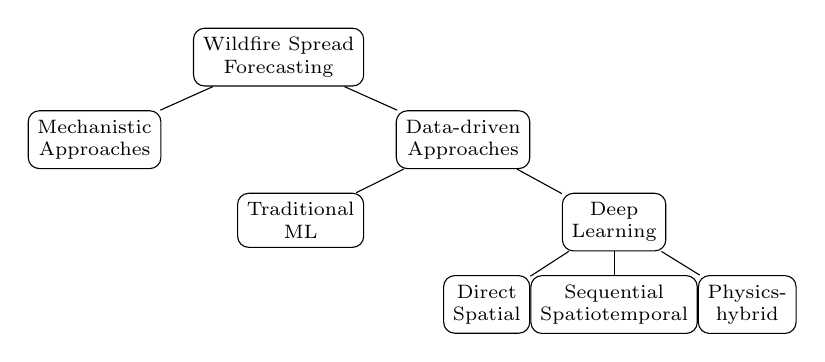
\begin{tikzpicture}[
        node distance=0.3cm and 0.4cm,
        every node/.style={
            draw,
            rounded corners,
            font=\scriptsize,
            align=center,
            minimum width=0.1cm,
            minimum height=0.1cm
        }
    ]

        % Root
        \node (root) {Wildfire Spread\\Forecasting};

        % First level
        \node (mechanistic) [below left=of root]
            {Mechanistic\\Approaches};

        \node (data) [below right=of root]
            {Data-driven\\Approaches};

        % Second level
        \node (ml) [below left=of data]
            {Traditional\\ML};

        \node (deep) [below right=of data]
            {Deep\\Learning};

        \node (spatial) [below left=of deep]
            {Direct \\ Spatial};
        \node (spatiotemporal) [below=of deep]
            {Sequential \\ Spatiotemporal};
        \node (physics) [below right=of deep]
            {Physics-\\hybrid};

        % Connections
        \draw (root) -- (mechanistic);
        \draw (root) -- (data);

        \draw (data) -- (ml);
        \draw (data) -- (deep);

        \draw (deep) -- (spatial);
        \draw (deep) -- (spatiotemporal);
        \draw (deep) -- (physics);
        

    \end{tikzpicture}

    \caption{Taxonomy of wildfire spread forecasting approaches.}
    \label{fig:taxonomy}
\end{figure}
\vspace{-1em}

\subsection{Comparative Analysis}

The deep-learning approaches in Figure~\ref{fig:taxonomy} differ in how they formulate wildfire forecasting, represent spatial and temporal information, combine input modalities, and incorporate domain knowledge. Direct spatial approaches focus on mapping the current fire and environmental state to a future fire distribution. For example, Next Day Wildfire Spread (NDWS) uses spatially aligned fire, weather, vegetation, drought, and terrain information to compare traditional machine-learning baselines with a neural network for next-day spread prediction~\cite{HUOT2022NDWS}. This formulation provides a strong spatial benchmark, but makes limited use of longer historical sequences.

Sequential spatiotemporal approaches explicitly model fire evolution across multiple observations. WildfireSpreadTS provides daily sequences of active fires together with fuel, weather, and topographic information, and supports models such as ConvLSTM and UTAE~\cite{GERARD2023WILDFIRESPREADTS}. These approaches can capture both spatial structure and temporal evolution and can combine multiple data sources, but they also introduce greater model and data complexity, including challenges from class imbalance and noisy observations. Physics-hybrid methods take a different approach by combining learned representations with known wildfire dynamics or physical constraints~\cite{VOGIATZOGLOU2025}. This can improve physical consistency, but requires additional domain assumptions and integration between learned and mechanistic components.

\begin{figure}[!ht]
    \centering

    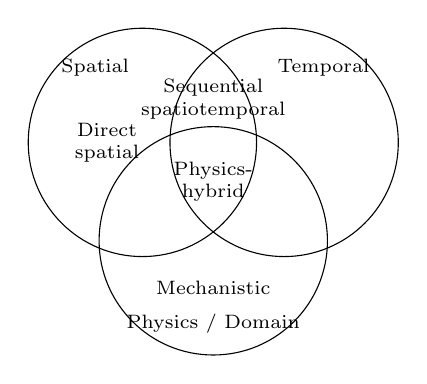
\begin{tikzpicture}[
        every node/.style={
            align=center,
            font=\scriptsize
        }
    ]

        \draw (-0.9,0.3) circle (1.45);
        \draw (0.9,0.3) circle (1.45);
        \draw (0,-0.95) circle (1.45);

        \node at (-1.5,1.25) {Spatial};
        \node at (1.4,1.25) {Temporal};
        \node at (0,-2) {Physics / Domain};

        \node at (-1.35,0.3) {Direct\\spatial};
        \node at (0,0.85) {Sequential\\spatiotemporal};
        \node at (0,-0.2) {Physics-\\hybrid};
        \node at (0,-1.55) {Mechanistic};

    \end{tikzpicture}

    \caption{Overlap among major wildfire forecasting approaches.}
    \Description{Venn diagram showing overlap among major wildfire forecasting approaches.}
    \label{fig:venn}
\end{figure}

Recent direct spatial methods also differ in how they represent and combine multimodal environmental information. FU-NetCastV2 uses a U-Net-based CNN with consecutive fire perimeters, satellite imagery, terrain, and weather data~\cite{KHENNOU2023100101}, while Shadrin et al.~\cite{Shadrin_Illarionova_Gubanov_Evteeva_Mironenko_Levchunets_Belousov_Burnaev_2024} similarly investigate multimodal inputs for wildfire spread prediction. WFNet further explores hierarchical spatial feature representation and multimodal fusion within a convolutional architecture~\cite{Jiang_Qiao_Su_Li_Meng_Wu_Quan_Wang_Wang_2023}. Together, these studies show that direct spatial approaches differ not only in architecture, but also in how heterogeneous environmental information is represented and fused.

\begin{table}[!ht]
\centering
\caption{Comparison of the three deep-learning wildfire forecasting approaches in Figure~\ref{fig:taxonomy}.}
\label{tab:comparison}
\vspace{-1em}
\small
\begin{tabular}{@{}p{1.25cm}p{1.65cm}p{1.85cm}p{2.35cm}@{}}
\hline
\textbf{Approach} &
\textbf{Prediction / Inputs} &
\textbf{Modeling} &
\textbf{Main Trade-off} \\ \hline

Direct spatial &
Future spread; spatial multimodal inputs &
CNN / spatial representation &
Strong spatial mapping; limited temporal dynamics \\

Sequential spatiotemporal &
Multi-step or next-day spread; temporal multimodal inputs &
ConvLSTM, attention, temporal models &
Captures fire evolution; higher data and model complexity \\

Physics-hybrid &
Spread or fire-front evolution; data and physical information &
Learned model with physical constraints &
Improved physical consistency; requires domain assumptions \\ \hline

\end{tabular}
\vspace{-1.5em}
\end{table}

\subsection{Project Positioning}

Our project focuses on the direct spatial approach to next-day wildfire spread forecasting. Existing work demonstrates that convolutional models can combine fire state with multimodal environmental information, including satellite imagery, weather, and terrain \cite{KHENNOU2023100101, Shadrin_Illarionova_Gubanov_Evteeva_Mironenko_Levchunets_Belousov_Burnaev_2024}. WFNet further demonstrates the potential of learned spatial representations and multimodal feature fusion for wildfire spread prediction~\cite{Jiang_Qiao_Su_Li_Meng_Wu_Quan_Wang_Wang_2023}. Additionaly, geospatial foundation models such as AlphaEarth Foundations provide pretrained representations of the physical environment that can be transferred to downstream mapping tasks \cite{brown2025alphaearth}. However, the usefulness of such representations for wildfire spread forecasting remains unclear.

Therefore, we investigate whether augmenting a conventional multimodal CNN with pretrained geospatial foundation-model representations provides additional information for next-day wildfire spread prediction. We use the same forecasting formulation and underlying architecture for both models, comparing a conventional multimodal baseline against an otherwise equivalent model augmented with foundation-model representations. This controlled comparison allows us to focus on the contribution of the pretrained representation rather than architectural complexity. Thus, our project positions itself at the intersection of direct spatial wildfire forecasting and geospatial representation learning, evaluating whether pretrained representations can provide useful information beyond conventional environmental inputs.


\bibliographystyle{ACM-Reference-Format}
\bibliography{bibliography.bib} 

\end{document}

